\documentclass[conference]{IEEEtran}

\usepackage{amsmath,amssymb}
\usepackage{booktabs}
\usepackage{float}
\usepackage{graphicx}
\usepackage[hidelinks]{hyperref}
\usepackage{xcolor}

\definecolor{implementedgreen}{RGB}{0,110,55}
\definecolor{plannedblue}{RGB}{30,80,160}
\definecolor{ongoingamber}{RGB}{145,79,0}
\newcommand{\implemented}{\textcolor{implementedgreen}{\textbf{Implemented}}}
\newcommand{\planned}{\textcolor{plannedblue}{\textbf{Planned}}}
\newcommand{\ongoing}{\textcolor{ongoingamber}{\textbf{Ongoing}}}

% Keep the wide acceptance artifacts together in their source order. IEEEtran
% otherwise limits the number of double-column floats placed at the page top.
\setcounter{dbltopnumber}{4}
\renewcommand{\dbltopfraction}{0.98}
\renewcommand{\dblfloatpagefraction}{0.90}
\setlength{\dbltextfloatsep}{8pt plus 2pt minus 2pt}

\title{Trajectory-Aware Reinforcement Learning for
Autonomous Tractor–Semitrailer Reverse Docking}

\author{
  \IEEEauthorblockN{Nandan Prince, Chris Pedretti}
  \IEEEauthorblockA{MSML 642, Group 20}
  \IEEEauthorblockA{Phase 2 Report : Nov 26, 2026}
  % \and
  % \IEEEauthorblockN{
  % \IEEEauthorblockA{MSML 642, Group 20}
}

\begin{document}
\maketitle

\begin{abstract}
Phase 1 established an operational two-dimensional Gymnasium task,
a configuration-generated three-dimensional MuJoCo model, and the first
closed-loop control vertical slice for autonomous tractor--semitrailer reverse
docking. Both plants share a versioned vehicle definition and controller
contract. The 2D environment supplies a path-relative observation, fixed
reverse speed, bounded steering-rate action, collision and jackknife events,
and a reproducible success condition. A trajectory-error linear quadratic
regulator (LQR) and a basic nonlinear model predictive controller (NMPC) now
drive this environment end to end. From a deliberately perturbed straight-path
start, both controllers reach the docking success event in the compact
scenario without collision or jackknife. These two runs establish software
integration and closed-loop authority. Phase 2 adds a replayable PPO
training pipeline and an open-bay condition for studying reverse stability
and path tracking. From a farther, laterally perturbed start, an early PPO
checkpoint jackknifed, while the final checkpoint reversed past the docking
target and exited the workspace. The experiments show progress in sustained
reversing. On a gentle curve, a selected PPO checkpoint achieved docking
and succeeded in 15 of 20 nearby-start trials. The final checkpoint
timed out on the training curve. The effect of path guidance remains to be
established.
\end{abstract}

\begin{IEEEkeywords}
tractor--semitrailer, reverse docking, Gymnasium, MuJoCo, linear quadratic
regulation, nonlinear model predictive control, proximal policy optimization
\end{IEEEkeywords}

\section{Introduction}

The project objective is to reverse one tractor and one conventional
semitrailer into a loading bay without collision or jackknife. The planned
study compares a trajectory-relative Proximal Policy Optimization (PPO)
controller with NMPC under the same vehicle, action, observation, task, and
evaluation definitions. The required experimental platform is a fast planar
Gymnasium environment; MuJoCo provides a later 3D transfer and demonstration
platform. This division follows the proposal while reducing the risk that the
learning and model-based methods are evaluated on different problems.

This report presents the implemented simulation stack and evaluates two
controllers behind a common interface. Perturbed closed-loop runs demonstrate
feedback control in the 2D task, while an open-loop cross-backend comparison
evaluates agreement between the kinematic and MuJoCo plants. The
trajectory-state formulation is motivated by Yan \emph{et al.}
\cite{yan2024trajectory}; the local NMPC direction is informed by Moradi and
Mehrandezh \cite{moradi2022nmpc}.

\section{Shared System Definition}

\subsection{Vehicle and control contract}

The planar state contains tractor axle position and heading, trailer heading,
steering angle, and speed. The trailer axle and hitch are reconstructed from
rigid geometry. For the canonical on-axle hitch, tractor yaw rate is
$\omega=v\tan\delta/L_t$ and trailer heading evolves as
\begin{equation}
  \dot{\psi}_r = \frac{v}{L_r}\sin(\psi_t-\psi_r),
\end{equation}
where $v<0$ during reverse motion. The simulator uses fixed-step RK4
integration. The research action is a normalized scalar mapped to bounded
steering rate; the reverse-speed target is fixed. Both LQR and NMPC use this
same action and the same $0.10\,\mathrm{s}$ controller period.

\begin{table}[t]
  \centering
  \caption{Compact baseline specification.}
  \label{tab:spec}
  \begin{tabular}{ll}
    \toprule
    Quantity & Frozen value \\
    \midrule
    Tractor wheelbase & $1.90\,\mathrm{m}$ \\
    Tractor body & $2.90\times1.00\,\mathrm{m}$ \\
    Trailer hitch-to-axle length & $4.00\,\mathrm{m}$ \\
    Steering angle / rate limits & $0.50\,\mathrm{rad}$ / $0.30\,\mathrm{rad/s}$ \\
    Reverse-speed target & $-0.20\,\mathrm{m/s}$ \\
    Controller period & $0.10\,\mathrm{s}$ \\
    Jackknife threshold & $45^\circ$ \\
    Docking pose tolerance & $0.10\,\mathrm{m}$ and $3^\circ$ \\
    \bottomrule
  \end{tabular}
\end{table}

\subsection{Reference path, observation, and task}

Reference paths are polylines ordered from dock target toward start.
Orthogonal projection supplies signed lateral error, progress, remaining
distance, and preview points. The bounded 21-element observation contains
lateral error, sine/cosine heading errors, articulation and articulation rate,
steering state, speed, remaining distance, docking-pose error, and three local
preview points. The Gymnasium environment evaluates docking success,
collision, jackknife, workspace exit, and timeout independently from reward.
Gymnasium's API checker passes for the registered \texttt{TrailerDocking-v0}
task.

\subsection{Programming setup}

The project is implemented as an installable Python package with versioned
dependencies and YAML-based vehicle, dock, and task configurations. Automated
verification includes 274 passing tests with $89.37\%$ branch-aware coverage.
Ruff linting and strict mypy type checking also pass. These checks cover the
shared vehicle core, kinematic and MuJoCo backends, Gymnasium API, task events,
controller integration, rendering, and artifact generation.

\subsection{Continuity with the proposal}

There are no material deviations from the proposed technical setup. The
project retains the custom 2D Gymnasium environment for controller development,
MuJoCo for the 3D demonstration and transfer stage, PPO as the principal
learning method, and NMPC as the model-based comparison method. The fixed
reverse-speed and steering-rate action, trajectory-relative observation,
collision and jackknife checks, and shared evaluation interface also remain
unchanged. LQR is included as an additional deterministic integration baseline
and does not replace the planned PPO--NMPC comparison. MuJoCo development was
completed earlier than originally scheduled, changing the implementation order
without changing the project scope.

\section{Implemented Controllers}

\subsection{Trajectory-error LQR}

The deterministic baseline numerically linearizes the verified RK4 kinematic
plant about straight motion at the configured reverse speed. Its local error
state contains trailer docking-point lateral error, tractor heading error,
trailer heading error, and steering angle. A discrete Riccati iteration
computes a feedback gain. The resulting physical steering rate is normalized
through the shared environment action. This controller primarily validates
sign conventions, tracking errors, actuation, and event handling; it is not
yet claimed to solve general curved docking.

\subsection{Basic NMPC}

The NMPC vertical slice predicts the nonlinear articulated model over 40
controller periods. Its objective penalizes trailer docking-point position and
heading errors, tractor heading, articulation, steering angle, and steering
rate. Steering rate is the sole decision input and speed remains at the fixed
reverse target. The CasADi/IPOPT implementation \cite{andersson2019casadi}
enforces initial state, discrete dynamics, steering-angle, steering-rate, and
articulation constraints, applies the first input, and warm-starts the next
solve. Collision is checked by the environment but is not yet an NMPC
prediction constraint.

The controller-facing contract includes the observation, physical state,
reference path, tracking errors, vehicle configuration, and step index. PPO
uses the Gymnasium observation and returns the same normalized one-element
steering-rate action through its controller adapter.

\section{Evaluation Protocol}

The closed-loop acceptance case uses a fixed straight reference path that is
independent of the reset pose. The vehicle begins $0.35\,\mathrm{m}$ laterally
displaced, with the tractor and trailer aligned at a $3^\circ$ heading offset.
Each controller must steer, develop articulation, reduce the path error, and
satisfy the configured docking-success conditions. Seed, configuration,
reference path, initial pose, and controller settings are deterministic.

The case is executed with the compact baseline. The figures show the initial
condition, the maximum-articulation point, and terminal docking success.
Numerical histories record lateral error, trailer-heading error, articulation,
and steering angle throughout each rollout. Both controllers use the same
vehicle, path, initial condition, fixed reverse speed, steering-rate limits,
task events, and success criteria.

This protocol is an engineering acceptance test. It does not randomize starts,
does not use a held-out scenario set, and does not equalize controller tuning
effort. Step count and accumulated reward are consequently reported as
descriptive run outputs, not as evidence that one method outperforms another.

\section{Results}

\subsection{Closed-loop acceptance}

Both controllers reached the configured success event without collision or
jackknife. The NMPC solver reported no failure. Table
\ref{tab:controller-results} reports the deterministic run outputs.

\begin{table*}[!t]
  \centering
  \caption{Perturbed-start closed-loop acceptance results. Heading and articulation are absolute magnitudes where indicated.}
  \label{tab:controller-results}
  \begin{tabular}{lrrrrrr}
    \toprule
    Controller & Steps & Time [s] & Final lateral [m] & Final heading [deg] & Max. articulation [deg] & Solver failures \\
    \midrule
    LQR  & 487 & 48.7 & $-0.0004$ & $0.0175$ & $6.59$ & 0 \\
    NMPC & 491 & 49.1 & $ 0.0128$ & $-0.0384$ & $12.79$ & 0 \\
    \bottomrule
  \end{tabular}
\end{table*}

Figures \ref{fig:lqr} and \ref{fig:nmpc} show that both methods produce a
visible steering correction from the configured initial perturbation.

\begin{figure*}[!t]
  \centering
  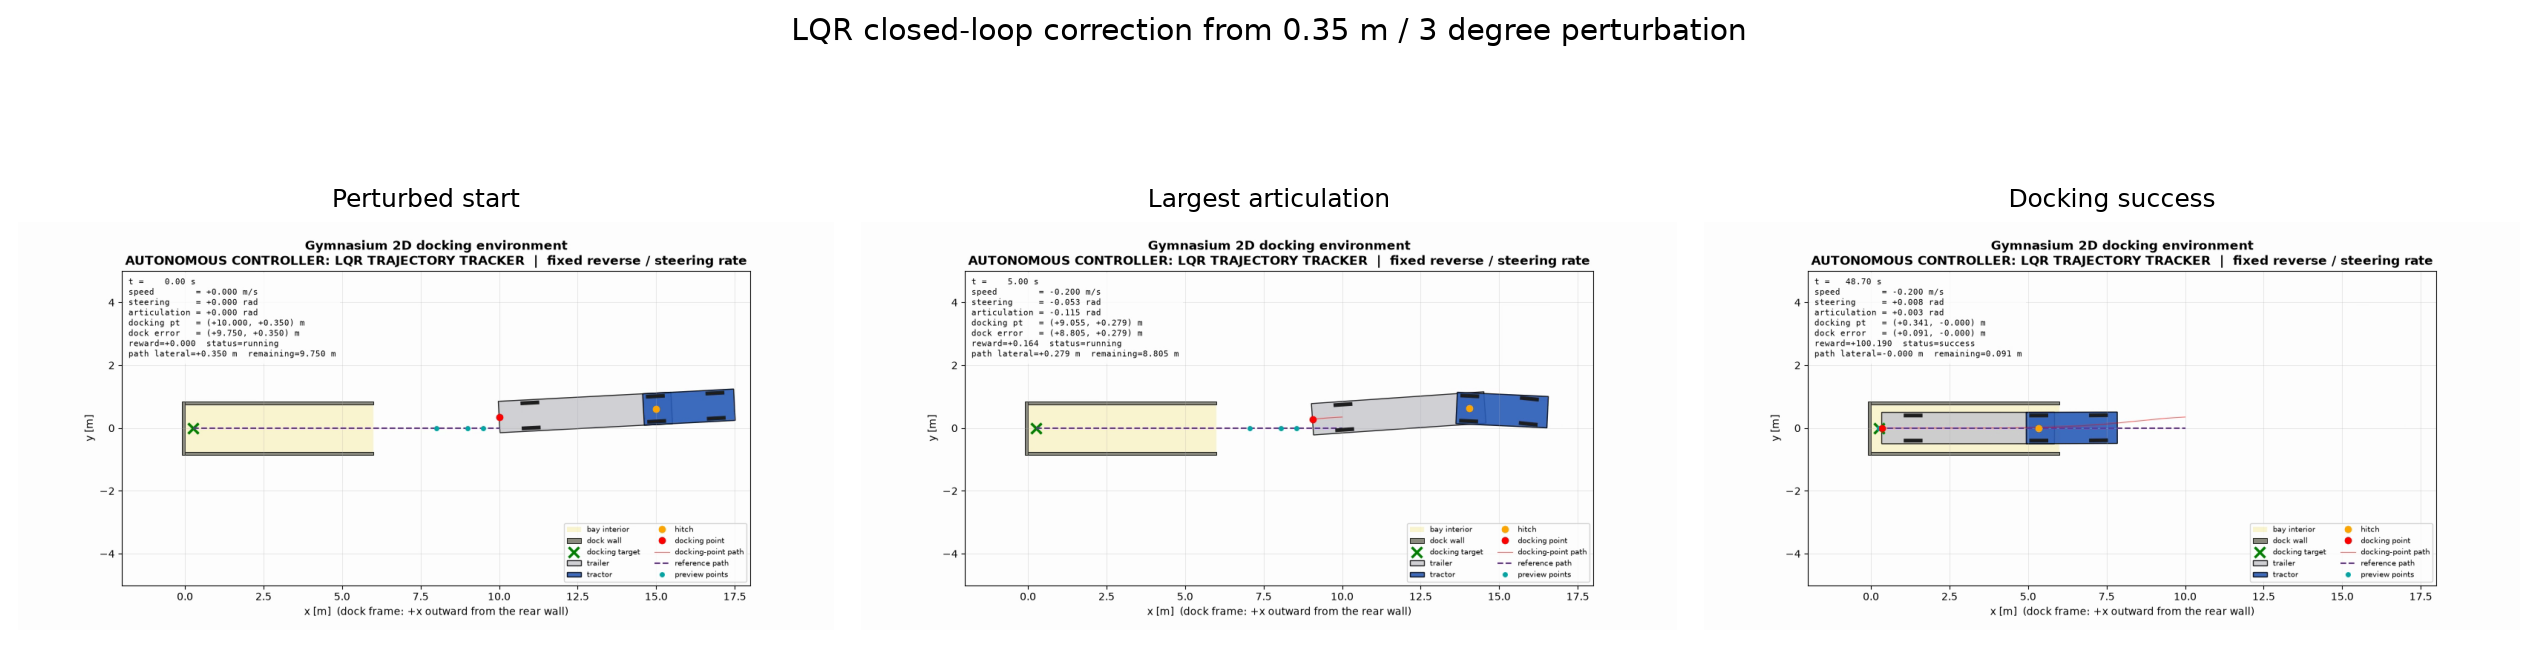
\includegraphics[width=\textwidth]{figures/lqr_compact_perturbed_tracking.png}
  \caption{LQR compact acceptance run. The middle panel is selected at the
  maximum-articulation step, demonstrating closed-loop correction from the
  perturbed pose.}
  \label{fig:lqr}
\end{figure*}

\begin{figure*}[!t]
  \centering
  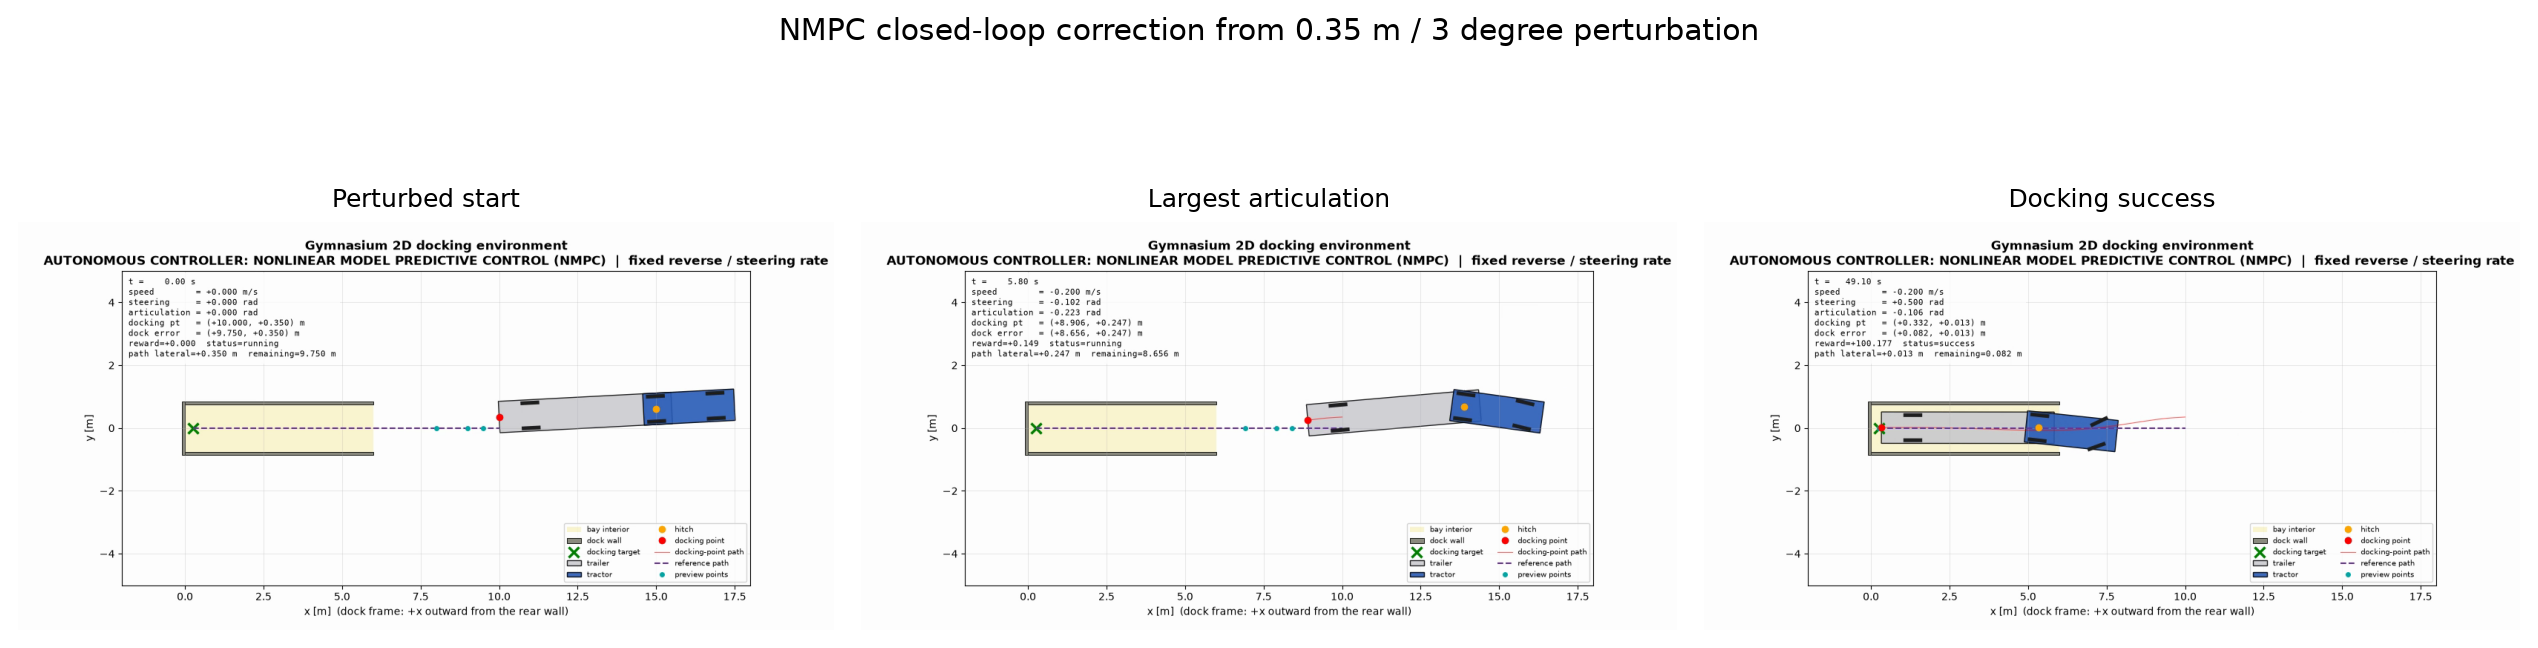
\includegraphics[width=\textwidth]{figures/nmpc_compact_perturbed_tracking.png}
  \caption{NMPC compact acceptance run using the same path, initial
  perturbation, fixed reverse speed, and steering-rate action as LQR.}
  \label{fig:nmpc}
\end{figure*}

The three-dimensional environment is also operational. Figure
\ref{fig:mujoco-straight} shows an offscreen MuJoCo rollout at the start,
midpoint, and rear-wall contact of a fixed straight-reverse command. The
generated scene contains the articulated tractor--trailer, loading bay,
Ackermann steering, driven rear wheels, hitch joint, cameras, and contact
geometry. This is evidence that the 3D plant and renderer run end to end; it is
not an LQR or NMPC result and does not yet demonstrate controller transfer.

\begin{figure*}[!t]
  \centering
  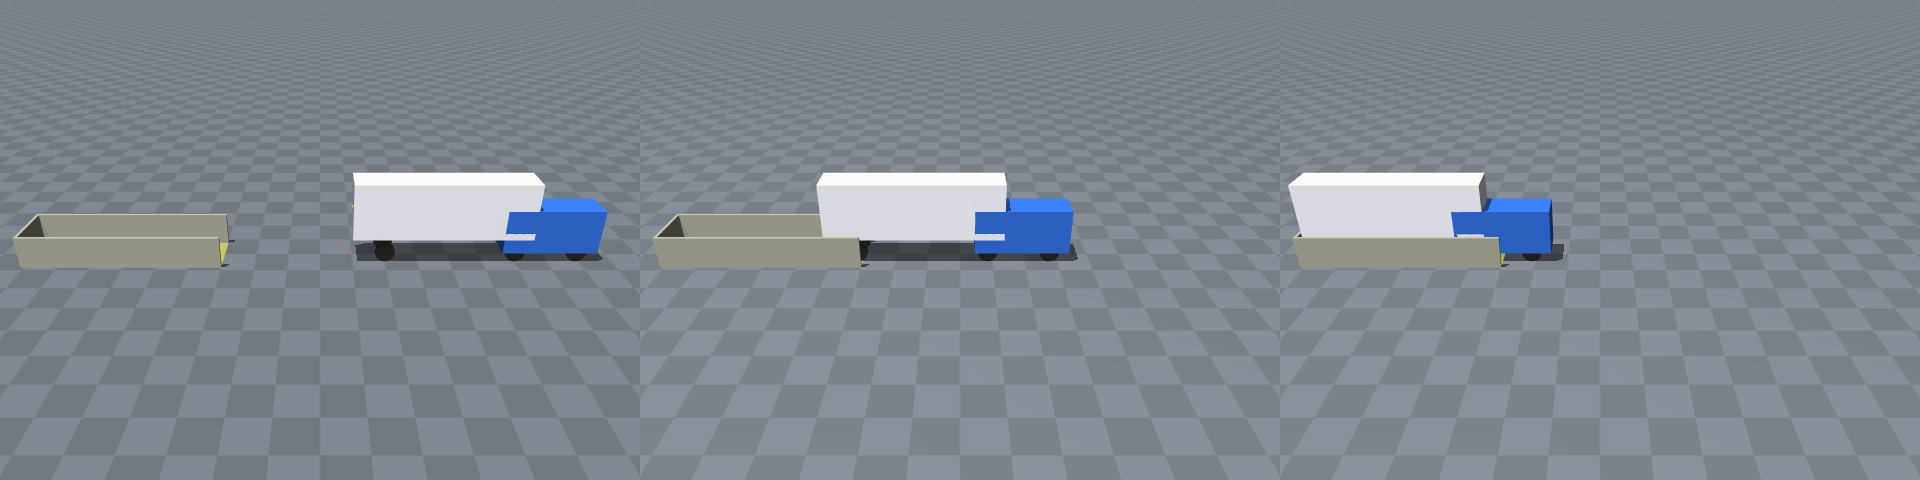
\includegraphics[width=\textwidth]{figures/mujoco_straight_reverse.png}
  \caption{MuJoCo 3D environment during a fixed straight reverse: start,
  intermediate motion, and trailer contact with the loading-bay rear wall.
  This is an environment demonstration, not a controller result.}
  \label{fig:mujoco-straight}
\end{figure*}

Figure \ref{fig:traces} shows the corresponding compact-run error and actuator
histories.

\begin{figure}[H]
  \centering
  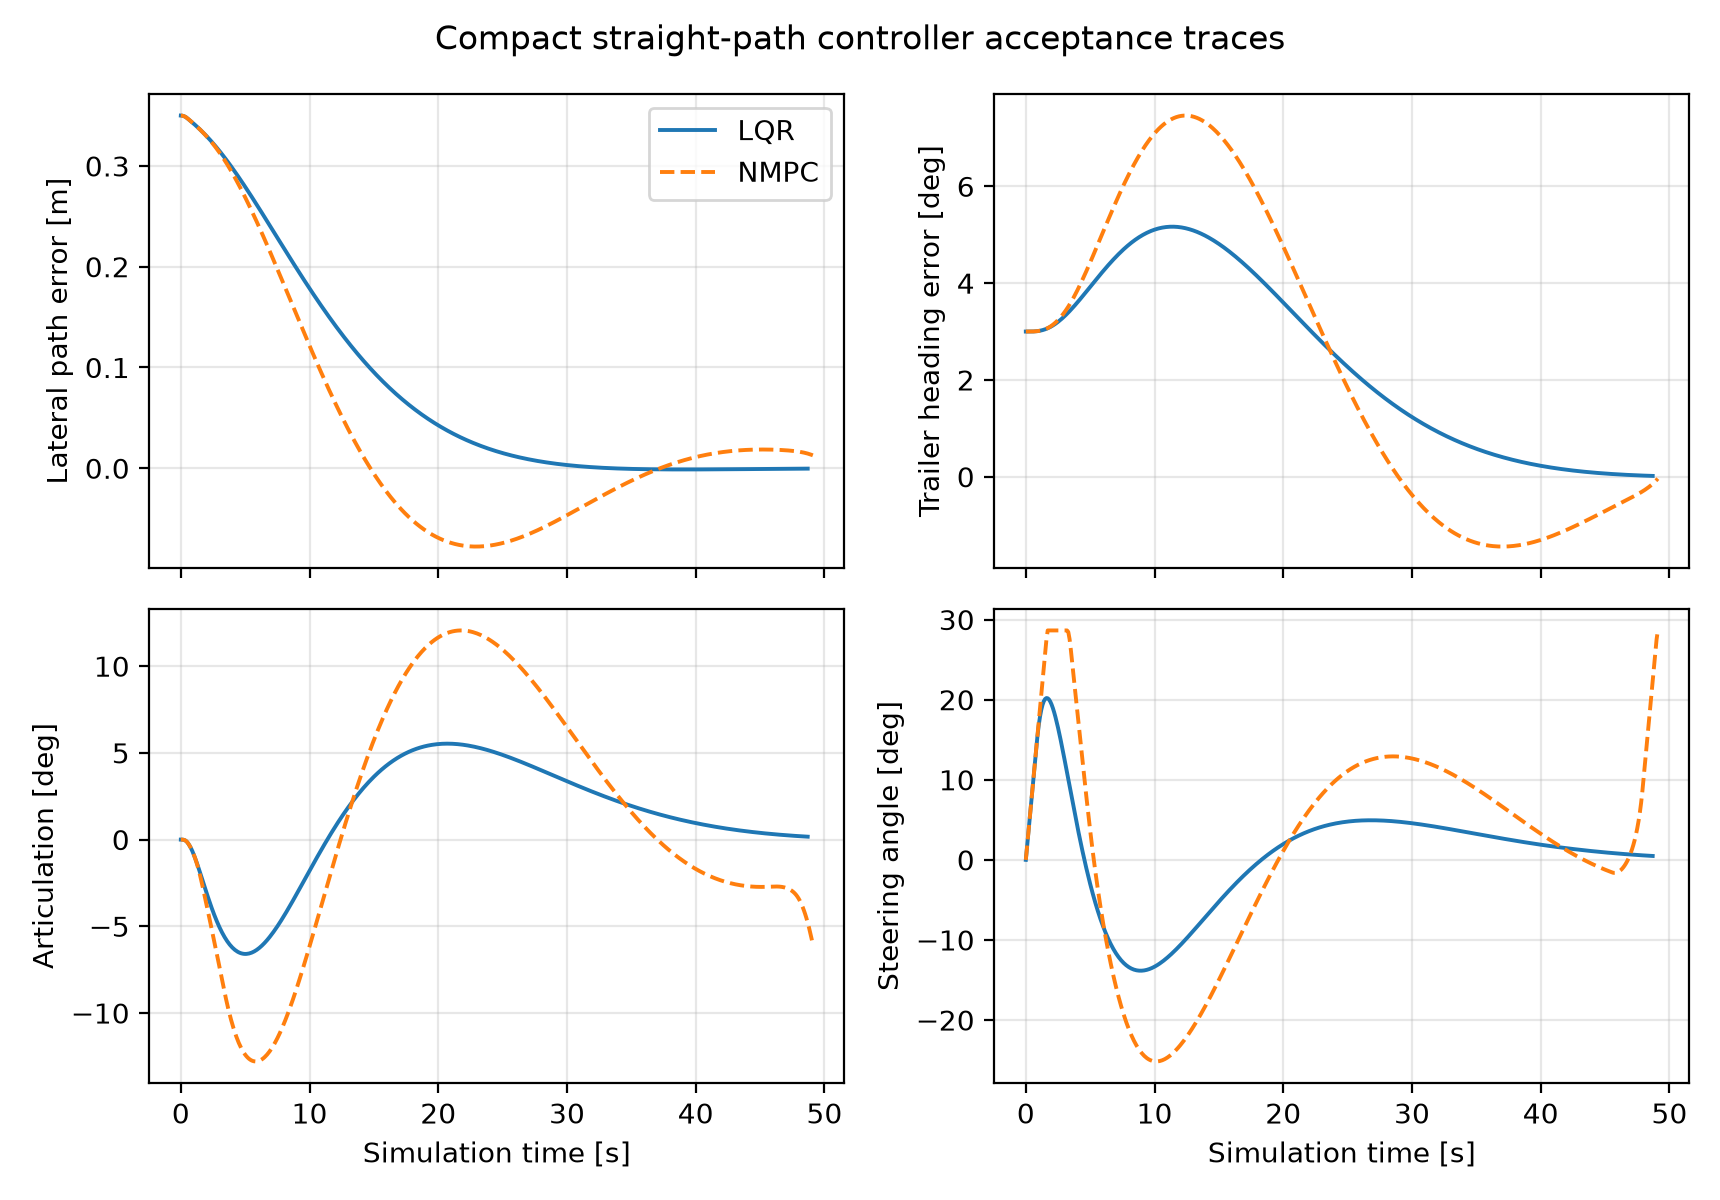
\includegraphics[width=\columnwidth]{figures/compact_controller_traces.png}
  \caption{Compact-run tracking and actuator histories. Different transients
  are visible, but this single tuned case is not a controller comparison.}
  \label{fig:traces}
\end{figure}

\subsection{Plant and software validation}

The implementation contains 274 passing tests with branch-aware coverage of
$89.37\%$ over the measured packages. Ruff linting and strict mypy checks pass.
Tests cover analytic derivatives, forward/reverse and constant-steering motion,
articulation response, angle wrapping, limits, rigid geometry reconstruction,
deterministic replay, timestep convergence, path projection, observation
bounds, safety events, Gymnasium API behavior, controller integration, video
export, MuJoCo model construction, and cross-backend trajectories.

The same 150 open-loop commands were applied to both plants over a
15-second reverse S-maneuver. The maximum tractor-position gap was
$0.008\,\mathrm{m}$ and the maximum articulation gap was
$0.0009\,\mathrm{rad}$. Figure \ref{fig:parity} is plant-parity evidence, not
controller-transfer evidence. The MuJoCo model is generated from the shared
configuration and exposes the same state and command contract; MuJoCo supplies
rigid-body dynamics and contacts \cite{todorov2012mujoco}.

\begin{figure}[H]
  \centering
  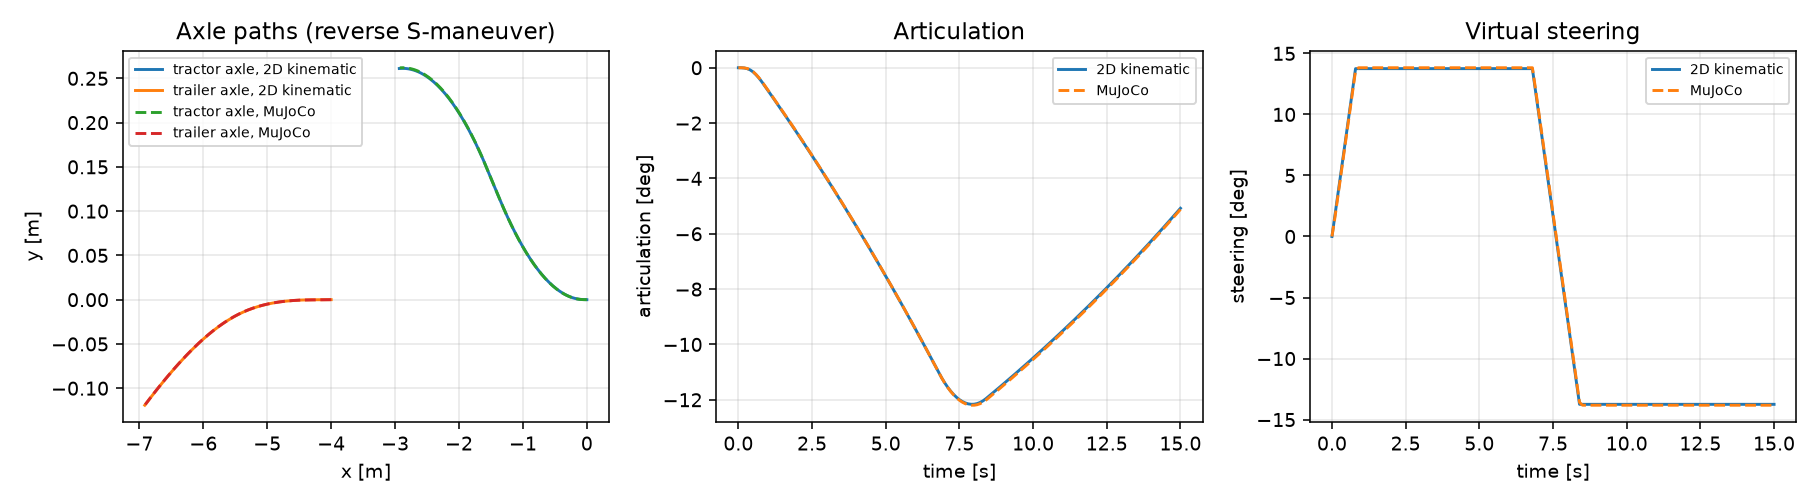
\includegraphics[width=\columnwidth]{figures/parity_2d_vs_mujoco.png}
  \caption{Open-loop low-speed comparison between the kinematic and MuJoCo
  plants under the same reverse command sequence.}
  \label{fig:parity}
\end{figure}

\section{Phase 2: PPO Training and Path Tracking}

\subsection{PPO Policy and Training}
We use the Stable-Baselines3 implementation of clipped PPO with a
multilayer perceptron actor and critic
\cite{schulman2017ppo,raffin2021sb3}. The path-guided policy takes the
normalized 21-element observation defined above. The three preview points
are $0.5$, $1.0$, and $2.0\,\mathrm{m}$ ahead in the reverse traversal
direction, expressed in the trailer frame. The policy outputs one
normalized steering-rate action in $[-1,1]$, scaled to a
$0.30\,\mathrm{rad/s}$ limit. The controller steps every
$0.10\,\mathrm{s}$ at a fixed reverse-speed target of $-0.20\,\mathrm{m/s}$.
The policy has no authority to stop or pull forward.

The goal-only pilot preserves the observation vector size and masks
path-relative lateral and heading errors, distance remaining along the
reference, and preview coordinates. Both ablation conditions retain
vehicle-state and dock-goal features and normalize goal positions by the
same workspace bounds. Both conditions use the same path-dependent reward,
so this ablation tests the policy's access to path observations.

The reported runs use 1,024-step rollouts, 256-sample minibatches,
10 optimization epochs per rollout, discount factor $\gamma=0.99$,
generalized advantage estimation with $\lambda=0.95$, and PPO clipping
parameter $\epsilon=0.2$.
The learning rate is $3\times10^{-4}$ for the initial training runs and
$10^{-4}$ for the matched recovery-reward comparison. A weights-only
warm start loads a prior policy and begins a new optimizer. During
training, actions are sampled. Checkpoint replay uses deterministic
actions and recorded validation seeds. Intermediate checkpoints highlighted
in the results were selected using the stated validation screens.

\subsection{Reward Design}
Let $\ell_t$ be the remaining arc length along the reference at the
orthogonal projection of the trailer rear point. Define
$\Delta\ell_t=\ell_{t-1}-\ell_t$, signed cross-track error $e_{y,t}$,
and trailer heading error $e_{\psi,t}$ in radians. Let
$d_t=|e_{y,t}|/\max(w_{\mathrm{bay}},1\,\mathrm{m})$.
The normalized articulation and steering rate are $\bar\alpha_t$ and
$\bar u_t$, each divided by its configured limit. The baseline compact
reward is
\begin{equation}
\begin{aligned}
r_t ={}& 10\Delta\ell_t-0.01-0.5d_t^2-0.2e_{\psi,t}^2\\
       & {}-0.15\bar\alpha_t^2-0.02\bar u_t^2+r_{\mathrm{event},t}.
\end{aligned}
\label{eq:ppo-reward}
\end{equation}
The event terms add $+100$ for a dock, $-100$ for collision or jackknife
per triggered event, and $-50$ for workspace exit. There is no separate
timeout term. There is no separate Euclidean-distance bonus for
approaching the dock. The progress term rewards advancing along the
reference, while the docking bonus requires the nominal pose tolerances
and complete trailer containment. The exploratory open bay retains the
painted target and docking criteria and removes physical dock walls.

The gated-progress variant scales only the positive progress term in
\eqref{eq:ppo-reward} by $[1+(e_{y,t}/0.30\,\mathrm{m})^2]^{-1}$.
The recovery variant retains that gate and adds
$5q_t(d_{t-1}-d_t)$, where $q_t=1$ if normalized error decreases or is
unchanged and $q_t=2$ if it grows. This adds immediate feedback for
correcting cross-track error. Both variants preserve the docking bonus
and event rules.

\subsection{Observed progress}
From an aligned start, PPO recorded 10 docks in 416 sampled training
episodes over 200,704 steps. There were 80 jackknifes among the first 81
episodes and none among the 85 episodes completed after step 150,000.
The final deterministic policy overshot the target. In two subsequent
runs with lateral offsets up to $0.15\,\mathrm{m}$ and heading offsets up to
$2^\circ$, the final policies docked in zero of 20 validation episodes each.
The 100,352-step run exited the workspace in every validation episode;
the 200,704-step run jackknifed in every validation episode.

Figure~\ref{fig:ppo-checkpoints} shows replay snapshots from a separate
200,704-step run that initialized PPO from the final aligned checkpoint.
The trailer began $8.0\,\mathrm{m}$ beyond the opening, $0.50\,\mathrm{m}$
off the straight centerline, with zero heading offset and articulation.
On this fixed start, the 20,000-step checkpoint jackknifed after 375 steps.
The final checkpoint sustained the reverse maneuver for 810 steps before
crossing the rear workspace boundary. The final policy failed to dock on
all 20 repetitions of this start. Sustained motion from a lateral offset
is evidence of progress on reverse control; heading, tracking, and docking
accuracy require further validation across starts.

\begin{figure*}[!t]
  \centering
  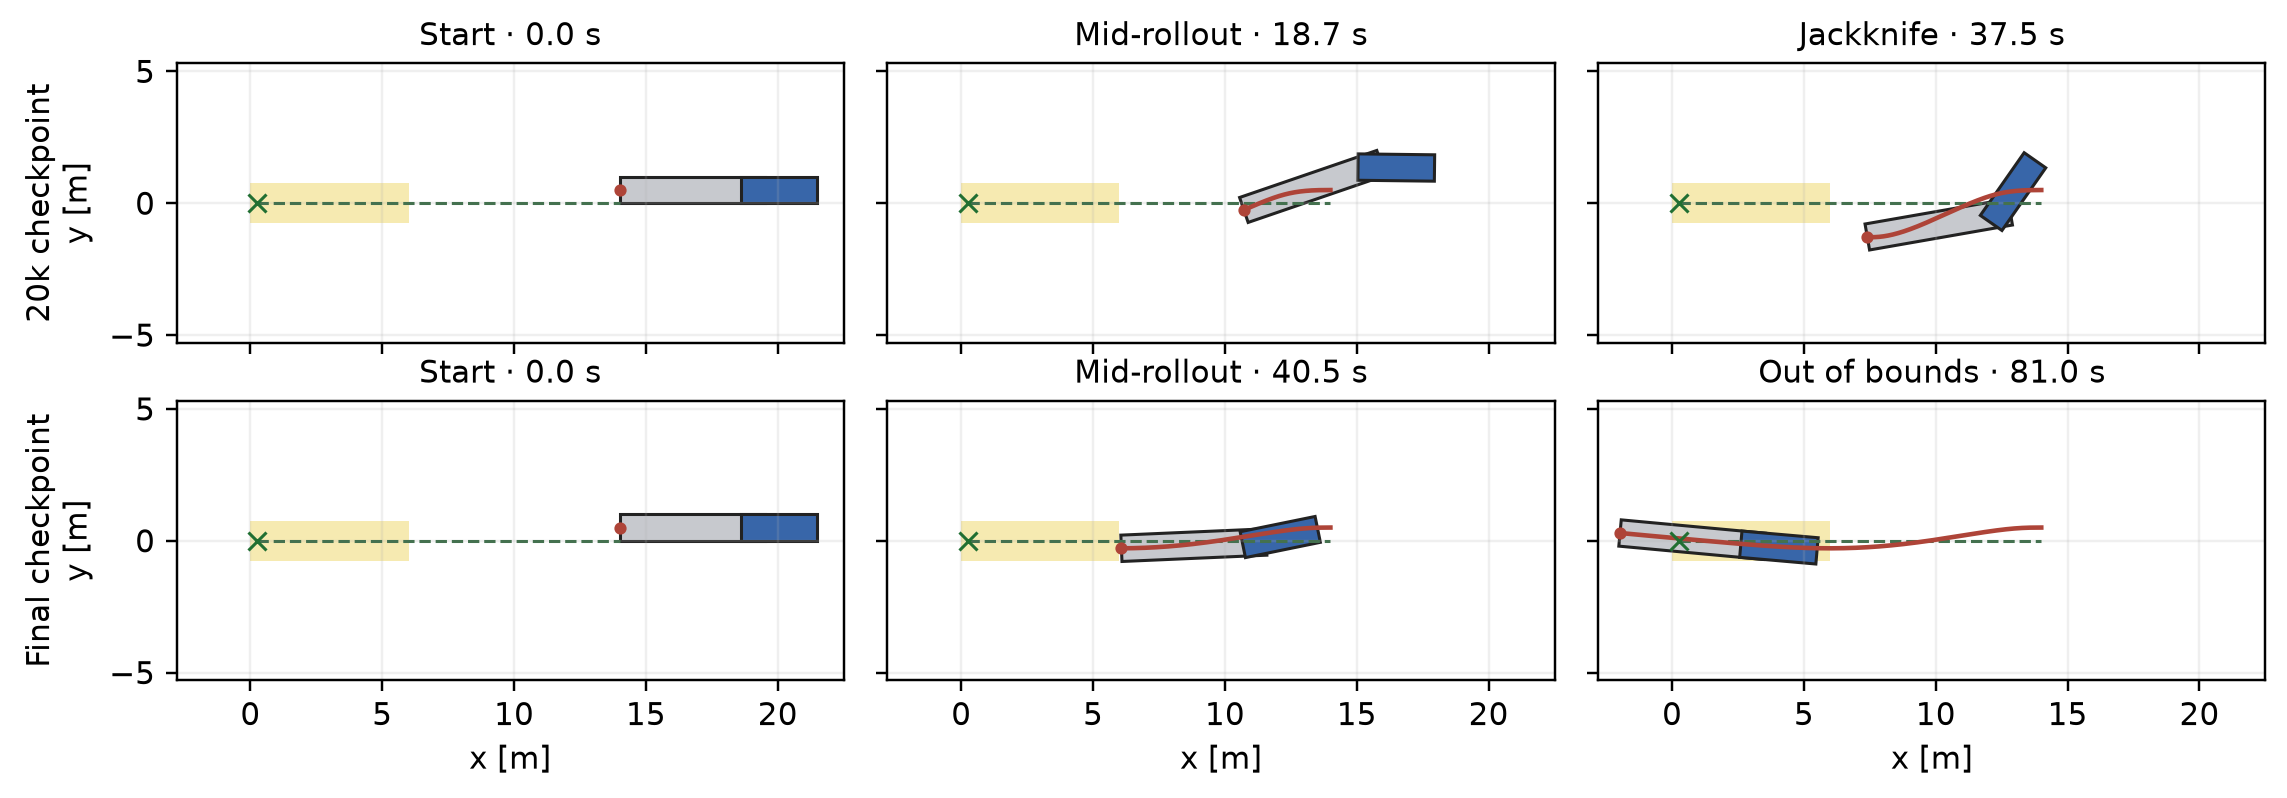
\includegraphics[width=0.98\textwidth]{figures/ppo_perturbed_replay.png}
  \caption{Deterministic 2D replays of the 20,000-step and final PPO
  checkpoints on the same $0.50\,\mathrm{m}$ lateral start offset. The shaded
  area marks the open bay, the dashed line is the reference, and the red
  trace follows the trailer rear point. Columns show reset, mid-rollout,
  and termination. These snapshots were reconstructed from saved policy
  checkpoints.}
  \label{fig:ppo-checkpoints}
\end{figure*}

\subsection{Gentle-curve PPO experiment}
The curved experiment uses the same open bay, fixed start, and version-1
reward as the farther-start straight-reference run. The gentle cubic
reference connects the trailer tail, $8.0\,\mathrm{m}$ beyond the bay opening
and $0.50\,\mathrm{m}$ off-center, to the docking target. PPO used the final
aligned policy as a weights-only initialization and completed 200,704
environment steps with training seed 0 and a 900-step episode limit.
Of 255 sampled training episodes, 36 docked, 170 exited the workspace,
46 jackknifed, and three timed out. The docking fraction declined over
training, from 22 of the first 64 episodes to zero of the last 50
(Fig.~\ref{fig:ppo-curve-training}).

\begin{figure}[t]
  \centering
  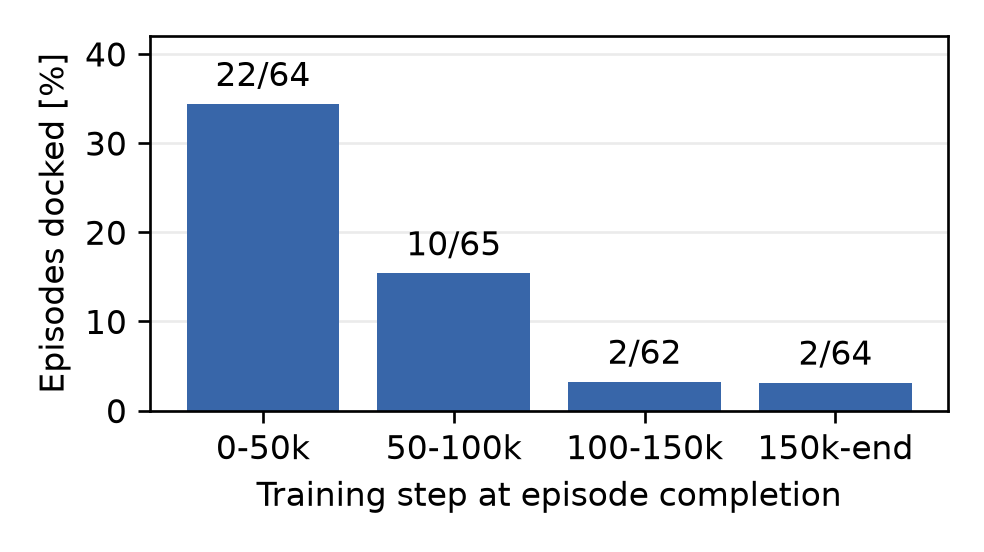
\includegraphics[width=\columnwidth]{figures/ppo_gentle_curve_training.png}
  \caption{Sampled gentle-curve training success grouped by the environment
  step at which each episode finished. Bar labels give docks over episodes.}
  \label{fig:ppo-curve-training}
\end{figure}

In deterministic replay, the 20,000- and 100,000-step checkpoints
docked on the training curve (Table~\ref{tab:ppo-curve}).
The 100,000-step checkpoint docked in 687 steps. Its mean absolute
lateral path error on approach was $0.082\,\mathrm{m}$, compared with
$0.852\,\mathrm{m}$ for the final policy. Approach error averages the
absolute path-relative lateral error over samples where the trailer rear
point has yet to pass the target longitudinal position. The final policy
timed out in 20 evaluations of the same fixed start. Figure~\ref{fig:ppo-curve}
shows the successful intermediate replay and the regression in the final
replay.

\begin{table}[t]
  \centering
  \caption{Deterministic PPO Replay on the Fixed Gentle Curve}
  \label{tab:ppo-curve}
  \begin{tabular}{lrrr}
    \toprule
    Policy & Outcome & Steps & Error [m] \\
    \midrule
    Initialization & Workspace exit & 806 & 0.097 \\
    20,000 steps & Docked & 692 & 0.210 \\
    100,000 steps & Docked & 687 & 0.082 \\
    Final & Time limit & 900 & 0.852 \\
    \bottomrule
  \end{tabular}
\end{table}

\begin{figure*}[!t]
  \centering
  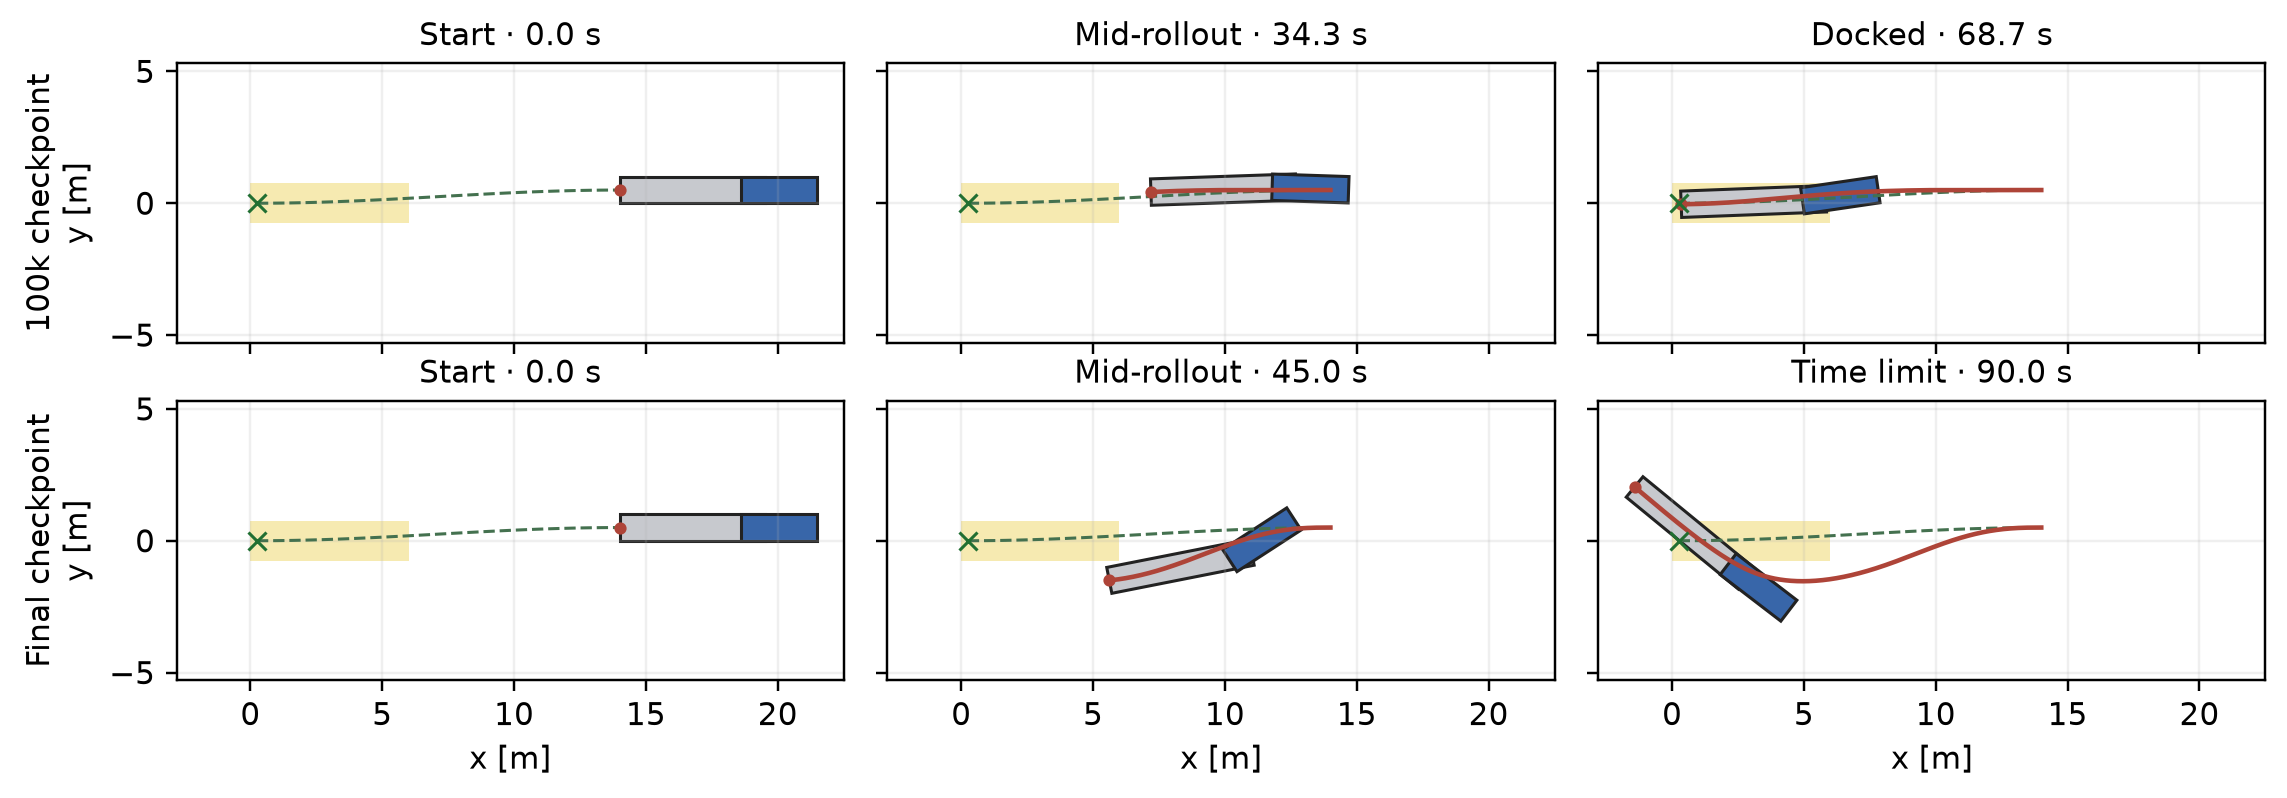
\includegraphics[width=0.98\textwidth]{figures/ppo_gentle_curve_replay.png}
  \caption{Deterministic 2D gentle-curve replays at reset, mid-rollout, and
  termination. The 100,000-step checkpoint docks. The final checkpoint
  passes the target and reaches the time limit. The dashed line is the
  reference and the red trace is the trailer rear-point trajectory.}
  \label{fig:ppo-curve}
\end{figure*}

The 100,000-step checkpoint was selected after inspecting replays on the
training curve. A paired exploratory diagnostic varied lateral starts over
$[0.40,0.60]\,\mathrm{m}$ and heading offsets over $\pm1^\circ$, resolving
the gentle reference from each start. The selected PPO checkpoint docked
in 15 of 20 trials and exited the workspace in the other five. LQR docked
in 20 of 20 on the same starts. This diagnostic uses one PPO training seed
and provides local robustness evidence. A matched path-guidance ablation
and a held-out PPO--NMPC comparison remain planned.

\subsection{Single-direction quarter-arc pilot}
To test a more visible curved approach, the trailer started tangent to
a $90^\circ$ arc of radius $10$--$11\,\mathrm{m}$, followed by a straight
final leg into the open bay. The guided PPO run used one turn direction,
small start variations, the existing path-based reward, and a 2,000-step
episode limit. It completed 400,384 training steps with zero docks in
625 completed episodes. Ends comprised 542 jackknifes, 80 workspace exits,
and three time limits. The final policy exited the workspace on all 20
validation starts. The checkpoint selected for greatest on-arc coverage
in a four-start replay screen was the 140,000-step policy. On the 20
validation starts it stayed within $0.5\,\mathrm{m}$ of the reference for
19.1\% of the arc on average before drifting out of that corridor or
terminating. The final policy covered 14.8\% by the same measure.
LQR docked on all 20 matched starts within 1,401 steps, establishing
feasibility for this scenario set.
The earlier mirrored observation pilots used 200,704 steps and a
900-step episode limit. Both final policies docked in zero of 20
validation episodes. The guided policy jackknifed on all 20 and the
goal-only policy recorded ten jackknifes and ten timeouts. The cap
was shorter than the verified maneuver time. A matched run with a
feasible cap is needed to isolate the effect of observation guidance
or training on one side.

\subsection{Short-arc tracking and docking}
The follow-up shortened the one-sided arc to $30^\circ$ at the same
$10$--$11\,\mathrm{m}$ radius. In 200,704 steps, guided PPO completed 421
sampled training episodes without a registered dock. In deterministic replay,
the intermediate 120,000-step checkpoint completed the arc within a
$0.5\,\mathrm{m}$ lateral corridor on all 20 validation starts, with
$0.027\,\mathrm{m}$ mean absolute lateral error on the arc. It then
deviated on the straight approach and exited the workspace in each case.
The final checkpoint covered 80.8\% of the arc within the corridor on
average and exited the workspace on all 20 starts. This pilot establishes
short-arc tracking for an intermediate checkpoint. Docking reliability
remains open.

\subsection{Reward tuning on the same short arc}
We retained the plant, reference, and start distribution and fine-tuned
from the 120,000-step short-arc checkpoint. The first run applied the
gated-progress variant to test whether concentrating progress rewards
near the reference improves the straight approach.

The exploratory gated run used a learning rate of $3\times10^{-4}$,
completed 200,704 additional steps, and recorded zero docks in 152
sampled episodes. All three checkpoints in Table~\ref{tab:reward-pilot}
exited the workspace on every validation start. The intermediate
fine-tuned checkpoint was selected by straight-approach error on a
four-start subset of the same validation set. The final checkpoint
tracked substantially worse than the initialization. A matched
ungated fine-tune at the same settings was not run, so the contribution
of the gate cannot be separated from the effect of additional PPO
updates.

\begin{table}[t]
  \centering
  \caption{Short-Arc Reward Pilot on 20 Matched Validation Starts}
  \label{tab:reward-pilot}
  \begin{tabular}{lrrr}
    \toprule
    Checkpoint & Arc [\%] & Straight MAE [m] & Docks \\
    \midrule
    Initialization & 100.0 & 0.95 & 0/20 \\
    Gated, +140k & 100.0 & 1.70 & 0/20 \\
    Gated, final & 59.4 & 12.85 & 0/20 \\
    \bottomrule
  \end{tabular}
\end{table}

Arc coverage measures the fraction traversed before the first lateral
error exceeding $0.5\,\mathrm{m}$ or termination. Straight-approach
MAE averages absolute lateral tracking errors over samples in the
longitudinal interval between the arc join and the target. The
recovery-reward trial adds a dense term for reduction in
absolute lateral error with a twofold multiplier when error grows.
The recovery condition and its gated-reward control use identical
initial weights, a new optimizer at $10^{-4}$, and a 60,000-step
budget. We evaluated docking and tracking outcomes on matched
validation starts.

The recovery-reward arm completed 60,416 steps at the planned learning
rate. Of 52 training episodes, 45 exited the workspace and seven
jackknifed. The initialization, selected 20,000-step fine-tuned
checkpoint, and final checkpoint each completed the arc within the
$0.5\,\mathrm{m}$ corridor on all 20 validation starts. No policy
docked. Mean straight-approach error was $0.95$, $0.93$, and
$5.78\,\mathrm{m}$, respectively. In all three replay sets, the tail
exceeded $0.5\,\mathrm{m}$ of lateral error on the straight approach and
never returned within $0.3\,\mathrm{m}$ during that approach. The
20,000-step checkpoint was selected on a four-start validation subset.
The matched gated-only control also completed 60,416 steps, with no
docks in 47 training episodes and no docks in 20 final validation
episodes. On matched starts, the recovery term reduced mean
straight-approach error relative to the control at 20,000 additional
steps ($0.93$ versus $2.26\,\mathrm{m}$). At 40,000 steps both means
were approximately $10.7\,\mathrm{m}$. At 60,000 steps the recovery and
control means were $3.02$ and $3.77\,\mathrm{m}$, respectively. In the final checkpoints,
the control had lower mean error ($3.72$ versus $5.78\,\mathrm{m}$).
Neither arm recovered into the specified lateral band or docked at
any checked checkpoint. This single-seed comparison shows transient
differences in tracking and no reliable recovery.

\subsection{MuJoCo replay}

The same trained policy can be evaluated on MuJoCo using the shared
observation and action interface. In a zero-shot software smoke check from
the aligned open-bay start, the 2D-trained final checkpoint executed on
both plants and exited the workspace after 604 steps in 2D and 605 steps
in MuJoCo. This establishes checkpoint execution in both plants on that
case. A matched transfer study remains pending.

\section{Progress and Limitations}

\begin{table}[t]
  \centering
  \caption{Current project status.}
  \label{tab:status}
  \begin{tabular}{p{0.62\columnwidth}p{0.25\columnwidth}}
    \toprule
    Component & Status \\
    \midrule
    Frozen vehicle/task contract & \implemented \\
    2D kinematic plant and Gymnasium task & \implemented \\
    MuJoCo vehicle, dock, and adapter & \implemented \\
    Reference-path and observation modules & \implemented \\
    Perturbed straight-path LQR acceptance & \implemented \\
    Perturbed straight-path NMPC acceptance & \implemented \\
    Curved and randomized controller study & \ongoing \\
    PPO training and checkpoint replay & \implemented \\
    Gentle-curve PPO docking pilot & \implemented \\
    Reliable perturbed-start PPO docking & \planned \\
    MuJoCo task-event parity and transfer & \planned \\
    Formal comparative experiments/ablations & \planned \\
    \bottomrule
  \end{tabular}
\end{table}

The curved and randomized study has completed exploratory 2D validation.
On the gentle-curve nearby-start set, the selected PPO checkpoint docked
in 15 of 20 trials and LQR docked in 20 of 20 on the same starts.
The $30^\circ$ pilot demonstrated arc tracking, with mean absolute
lateral error of $0.027\,\mathrm{m}$ for the selected checkpoint, but did
not yield docking. The quarter-arc and short-arc results identify
articulation and final alignment as separate failure modes. The PPO
experiments use one training seed per condition and inform the next
tests. The reported NMPC baseline has completed straight-path acceptance;
paired curved-path NMPC evaluation is pending. MuJoCo execution has
been checked for one PPO checkpoint.

The next gate is a frozen scenario suite containing straight, curved, and
randomized starts. A geometric or LQR baseline, NMPC, and PPO will then be run
with common seeds and saved run records. Metrics will include success,
collision, jackknife, terminal pose error, path error, articulation, control
effort, and compute time. The effect of path guidance will be tested with
matched starts, goals, and training budgets. Broader MuJoCo comparisons will
also require checks of contact and task-event consistency.

\section{Conclusion}

Phase 1 establishes the foundational simulation and control stack for
tractor--semitrailer reverse docking. The shared vehicle specification, planar
kinematic model, Gymnasium task, and MuJoCo environment are operational and
supported by automated verification. In the 2D environment, both the
trajectory-error LQR controller and the basic NMPC controller complete a
perturbed straight-path docking scenario through the common fixed-speed,
steering-rate control interface. The MuJoCo results demonstrate operational
3D vehicle motion and contact handling. Phase 2 adds PPO training and
checkpoint replay, with evidence of longer reverse rollouts in the open
bay, docking on a gentle curve at an intermediate checkpoint, and
checkpoint execution in MuJoCo.

The next experiments address reliable docking on perturbed and curved
starts, the benefit of path-relative guidance, and fair comparisons of PPO
and NMPC on identical held-out scenarios.

\bibliographystyle{IEEEtran}
\bibliography{references}

\end{document}
